\documentclass[nopagenumber,9pt]{beamer}

\mode<presentation> {
  \usetheme[]{CambridgeUS}
  %\useoutertheme{shadow}
  \setbeamercovered{transparent}
  \usecolortheme{seahorse}
%\usecolortheme{sidebartab}
%  \usefonttheme{structurebold}
  \useinnertheme{default}
\useinnertheme{rounded}
}
\usepackage{nicefrac}
\RequirePackage{amsmath,amsfonts,amsthm}
\newtheorem{Prop}{Proposition}

\usepackage{float}
\usepackage[english]{babel}
\usepackage{amsmath}
\usepackage[utf8]{inputenc}
\usepackage{times}
\usepackage{url}
\usepackage[T1]{fontenc}
%\usepackage{multirow}
\usepackage{color}
\newcommand{\mb}[1]{\mathbf{#1}}
\usepackage{graphicx}
\graphicspath{{./figure/}}
\usepackage{multirow}

\definecolor{dgreen}{RGB}{139,172,100}

\hypersetup{
  colorlinks = true,
  linkcolor = black
}
\makeatletter
\let\@mycite\@cite
\def\@cite#1#2{{\hypersetup{linkcolor=dgreen}[{#1\if@tempswa , #2\fi}]}}
\makeatother

\usepackage[ruled,vlined]{algorithm2e}
\usepackage{xcolor,colortbl}
\usepackage{rotating}
\usepackage{multirow}

\usepackage{tikz}
\usepackage{ulem}
\newcommand{\argmax}[2]{% 
\smash{\mathop{{\rm argmax}}\limits_{#1}}\,#2} 
\usepackage{stmaryrd}
\newtheorem{proposition}{Proposition}

% 
% \newcommand{\I}{\mathbb{I}}
% \newcommand{\E}{\mathbb{E}}
% \renewcommand{\P}{\mathbb{P}}
% \newcommand{\R}{\mathbb{R}}
% \newcommand{\bs}{\boldsymbol}
% \newcommand{\bbeta}{\boldsymbol{\beta}}
% \newcommand{\balpha}{\boldsymbol{\alpha}}
% \newcommand{\btheta}{\btheta}
% \newcommand{\bY}{\mathbf{Y}}
% \newcommand{\bX}{\mathbf{X}}
% \newcommand{\bZ}{\mathbf{Z}}
% \newcommand{\by}{\mathbf{y}}
% \newcommand{\bz}{\mathbf{z}}
% \newcommand{\ba}{\mathbf{a}}
% \newcommand{\bx}{\mathbf{x}}
% \newcommand{\bh}{\mathbf{h}}
% \newcommand{\bb}{\mathbf{b}}
% \newcommand{\bB}{\mathbf{B}}
% \newcommand{\bM}{\mathbf{M}}
% \newcommand{\bphi}{\boldsymbol{\phi}}
% \newcommand{\bpsi}{\boldsymbol{\psi}}
% \newcommand{\bpi}{\boldsymbol{\pi}}
% \newcommand{\btau}{\boldsymbol{\tau}}
% \newcommand{\Ecal}{\mathcal{E}}
% \newcommand{\GP}{\mathcal{GP}}
% \newcommand{\bxi}{\boldsymbol{\xi}}
% \newcommand{\brho}{\boldsymbol{\rho}}
% \newcommand{\bgamma}{\boldsymbol{\gamma}}
% \newcommand{\bsigma}{\boldsymbol{\sigma}}
% \newcommand{\nf}{n_e}
% \def\ee{{\mathbb E}}
% \newcommand{\dd}{\mathrm{d}}
% 
% %%%macros
% \newcommand{\yexpi}{y_{exp_i}}
% \newcommand{\bxf}{\bx^e}
% \newcommand{\byf}{\by^e}
% \newcommand{\Df}{D^e}
% \newcommand{\byc}{\by^c}


\usepackage{macros}

\newcommand{\ms}[1]{\boldsymbol{#1}}
\newcommand{\blue}{\textcolor{myblue}}
\definecolor{myblue}{RGB}{0,56,115}

\title[Sequential Designs]{Calibration of computer models}

%titre premiere page

\subtitle{Sequential Designs of Experiments}

\author[P. Barbillon]{ Pierre \textsc{Barbillon}}
\bigskip

\date{Fall 2023}

\subject{Séminaire}



\AtBeginSection[] {
 \begin{frame}<beamer>
   \frametitle{Outline}
   \tableofcontents[currentsection]
  \end{frame}
}

\AtBeginSubsection[] {
\begin{frame}<beamer>
   \frametitle{Outline}
   \tableofcontents[currentsection,currentsubsection]
 \end{frame}
}


\begin{document}

\begin{frame}
\titlepage
%\includegraphics[scale=.12]{AgroParisTech_-_logo.PNG}
%\vspace{-1.5cm}
%\begin{flushright}
% \includegraphics[scale=.1]{Logotype-INRA-transparent.png}
% \end{flushright}
\vspace{-1cm}
\centering
\begin{tabular}{ccc}
 
\includegraphics[scale=.08]{LogoUPSaclay.jpg}&
  
\includegraphics[scale=1.3]{agrologo.png}&
   
\includegraphics[scale=.1]{LogoINRAE.jpg}
\end{tabular}


\end{frame}



\section{Apprixmate calibration}

\begin{frame}
 \frametitle{Considered framework}
 
 Model $\mathcal{M}_2$:
$$\mathcal{M}_2  : \ \forall i \in \llbracket1,\dots,\nexp\rrbracket, \quad \yexpi = F(\boldsymbol{x}_i,\btheta) + \epsilon_i,$$
 
 \bigskip
 
 \textbf{Goal}: find DoNE in order to make $\pi(\btheta|\byexp,\byc,\bXexp,\Dc)=\pi^{C}(\btheta|\byexp,f(\Dc_M))$ as close as possible to $\pi(\btheta|\byexp)$ under a limited $N$.
 
 
 \bigskip
 
 \begin{beamerboxesrounded}{Extension to M4}
  Possible if a priori on the discrepancy function.
 \end{beamerboxesrounded}

\end{frame}


 \begin{frame}
 \frametitle{Posterior consistency}
 \begin{Prop}
\label{PropKL}
Under the following assumptions:
\begin{itemize}
\item $\pi(\btheta)$ has a bounded support $\Theta$, 
\item the code output $f(\textbf{x},\btheta)$ is uniformly bounded on $\mathcal{X}\times\Theta$,
\item the correlation function (kernel) of the GP surrogate is a classical radial basis function %\citep{Scha95b},
\item $f$ lies in the associated Reproducing Kernel Hilbert Space,
\item the covering distances $h_{\Dc_M}$ associated with the sequence of designs $(\Dc_M)_M$ tends to $0$ with $M\rightarrow\infty$,
\end{itemize}
then, we have:
 \begin{equation*}
\label{robust}
\lim_{M\to\infty}\textrm{KL}\big(\pi(\btheta|\byexp)||\pi^{C}(\btheta|\byexp,f(\Dc_M))\big)=0\,.
\end{equation*}
\end{Prop}
 
 \medskip
 
 
 where
 \begin{equation*}
h_{\Dc_M}=\max_{(\bx',\btheta')\in\mathcal{X}\times \Theta}\min_{(\bx_i,\btheta_i)\in \Dc_M}\Vert 
(\bx',\btheta')-(\bx_i,\btheta_i)\Vert\underset{M\to\infty}\longrightarrow 0 \,.
\end{equation*}
 
 
\end{frame}





  \begin{frame}
 \frametitle{Motivation for adaptive designs in calibration}
   Quality of calibration (Bayesian or ML) is affected by choice in the numerical design.
 \\
 \bigskip
  
  
$\bullet$ Calibration with unlimited runs of $f$
  \begin{center}
   \begin{figure}
    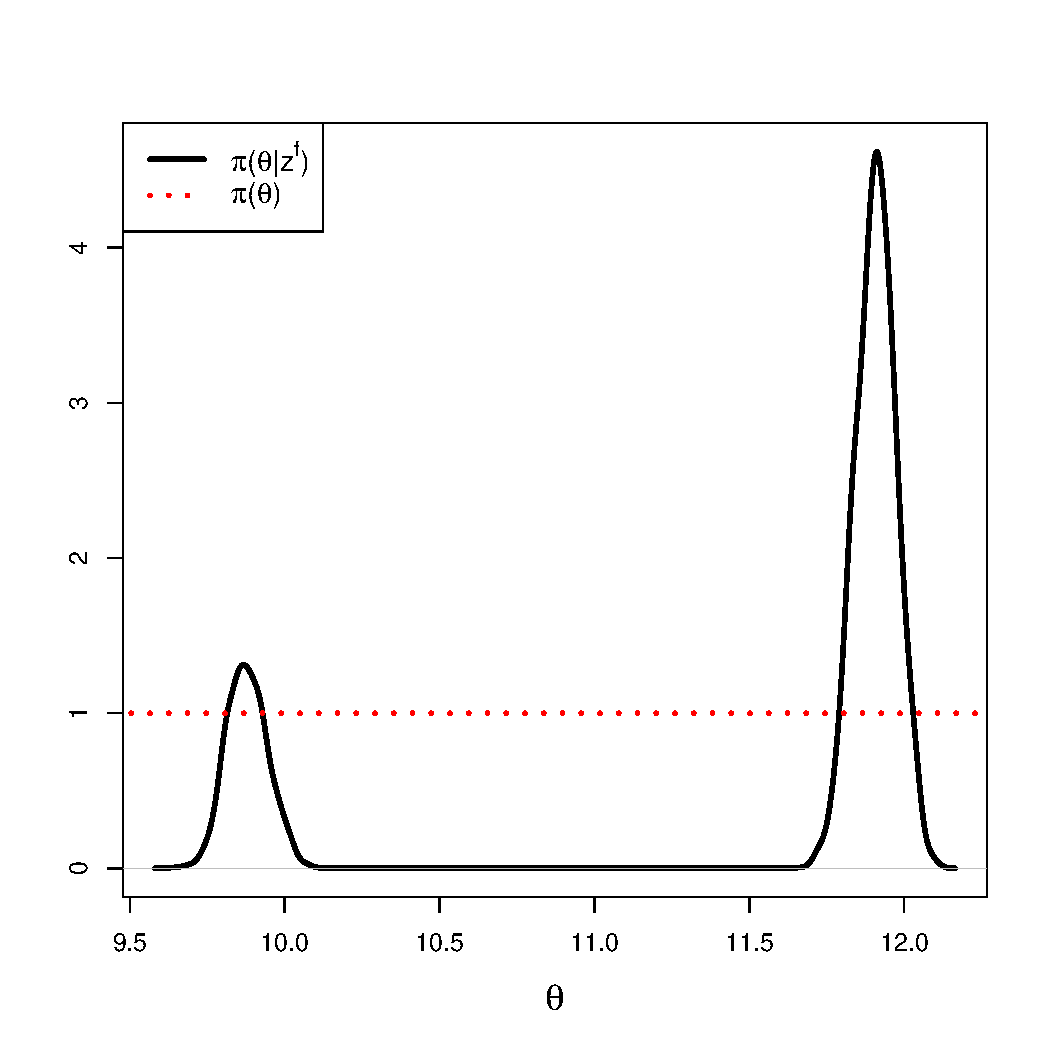
\includegraphics[scale=0.3]{calib_sans_biais_jouet_true.pdf}
   \end{figure}

  \end{center}

 \end{frame}

 
 \begin{frame}
  \frametitle{LHS maximin design}
  \begin{figure}
   \begin{center}
    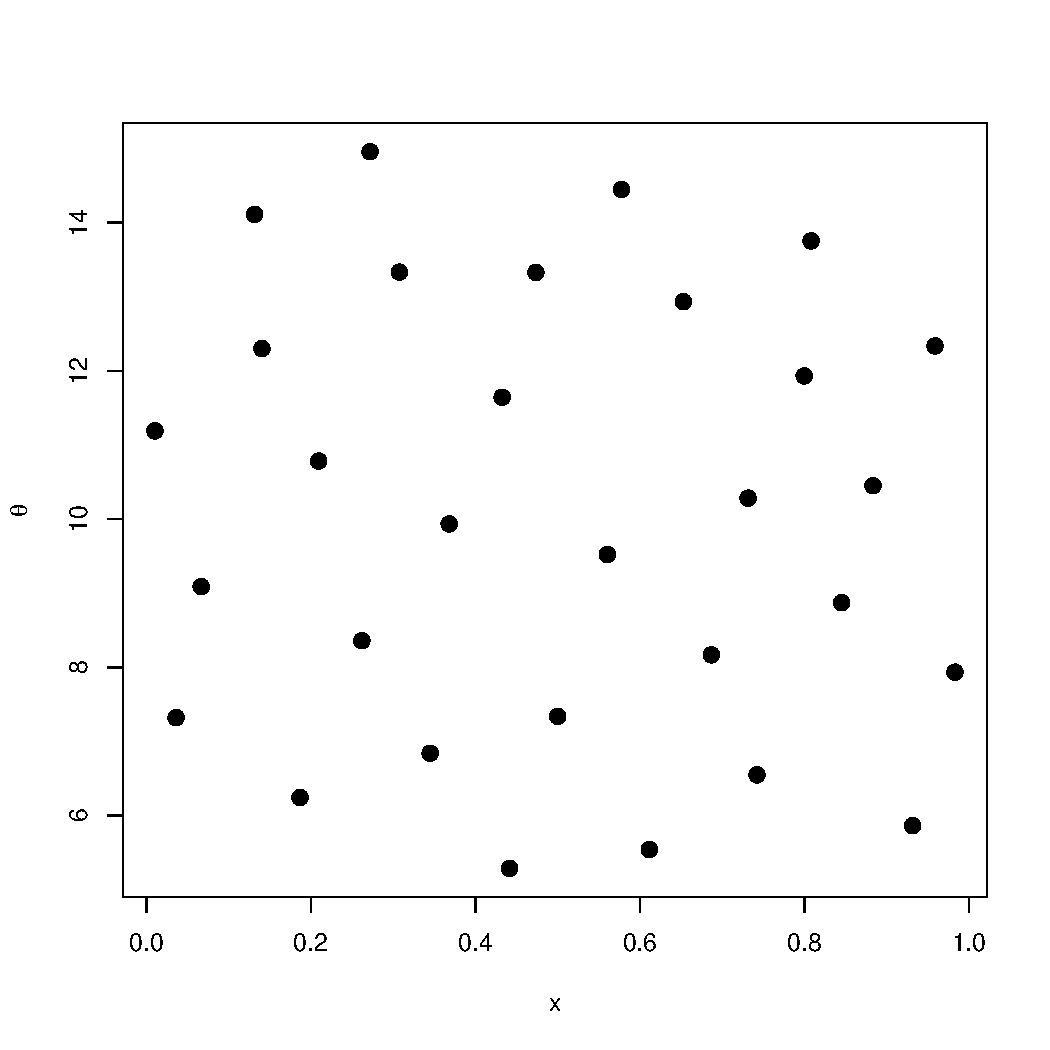
\includegraphics[scale=.3]{maximin.pdf}
   \end{center}

  \end{figure}

  
 \end{frame}

 
 
 \begin{frame}
 \frametitle{Motivation for adaptive designs in calibration}
 
$\bullet$ Calibration with emulator built from a design with $M=30$ calls to $f$

  \begin{center}
  \begin{figure}
   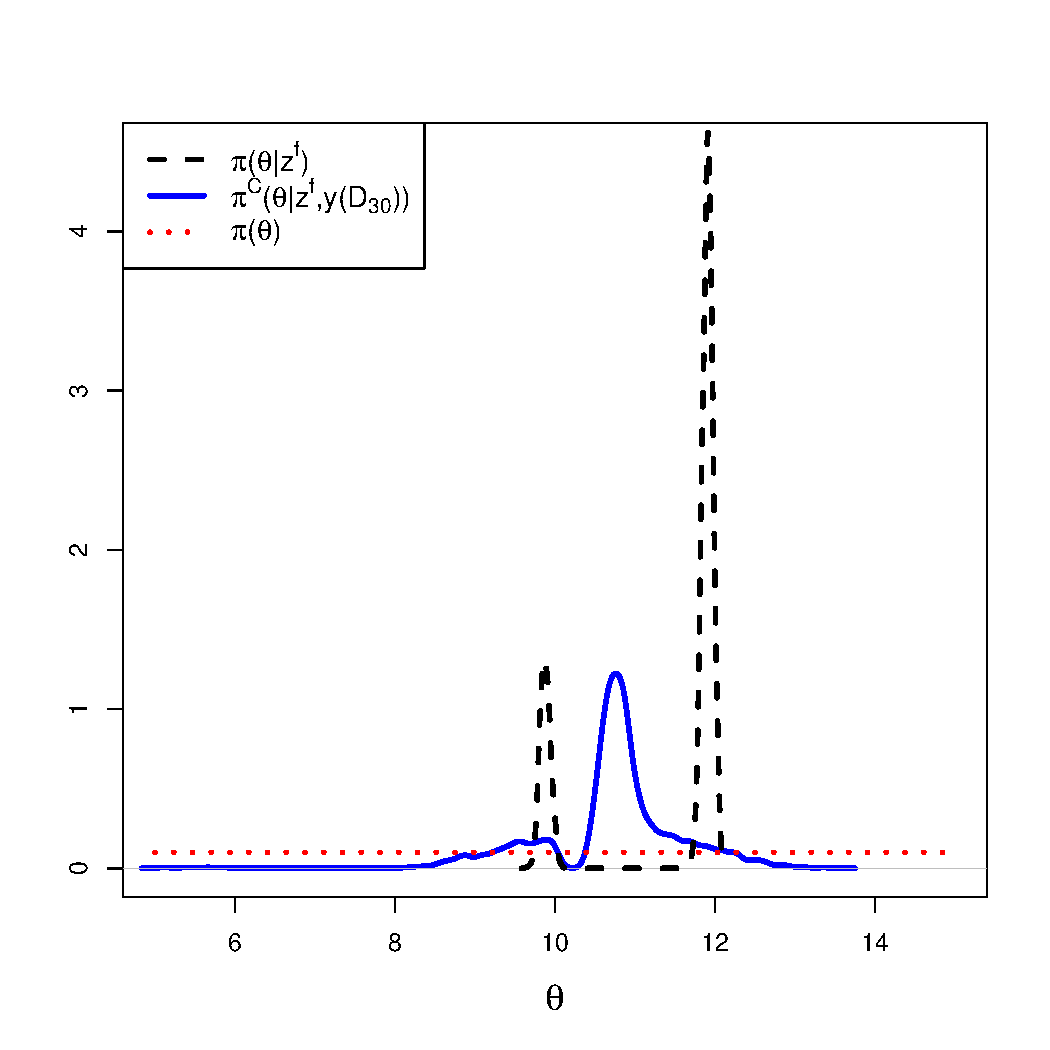
\includegraphics[scale=0.25]{calib_sans_biais_jouet_M30_072.pdf}
   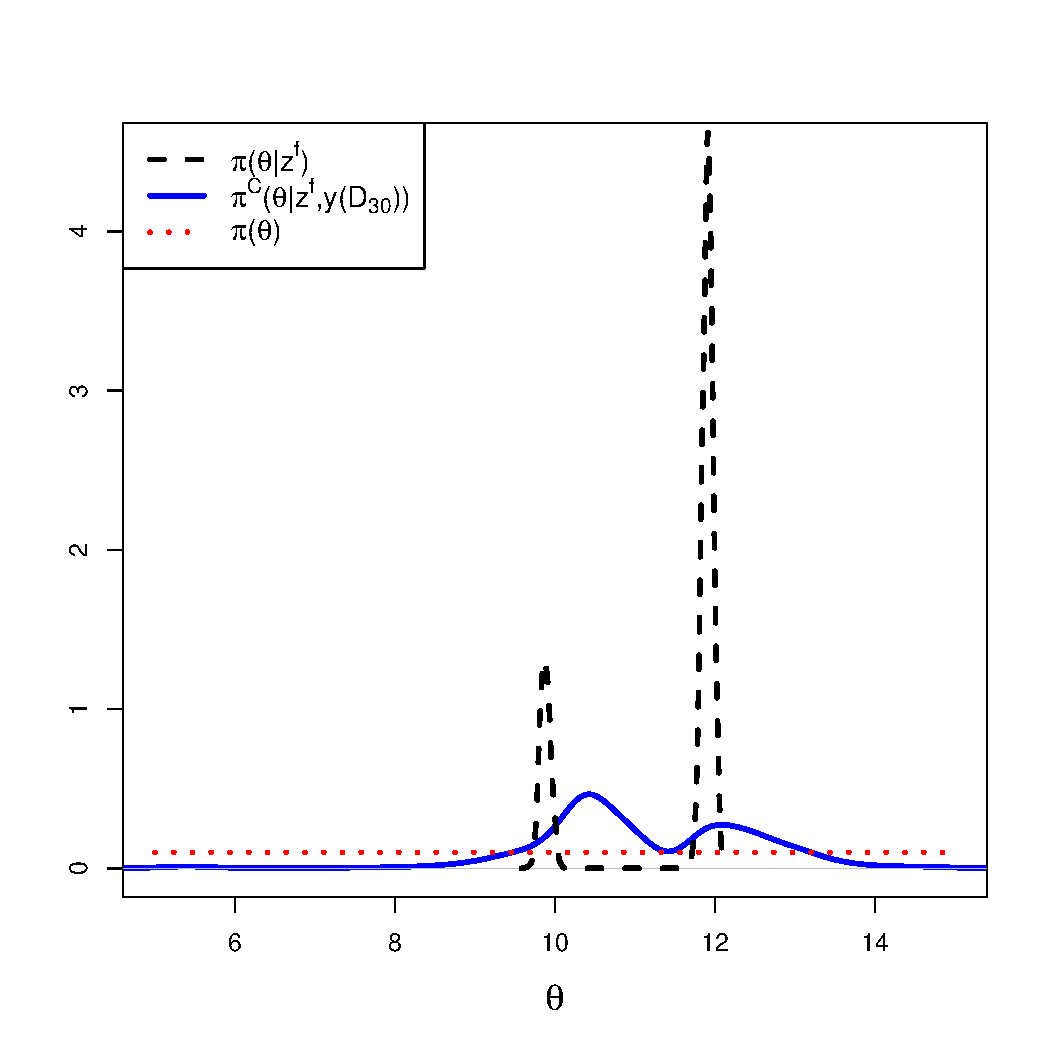
\includegraphics[scale=0.25]{calib_sans_biais_jouet_M30_062.pdf}
  \end{figure}
 
  \end{center}

  
%calibration  au sens du max de vrais

 
\end{frame}


\section{EGO enhanced design of numerical experiments for calibration}





\begin{frame}
 \frametitle{EI for calibration}
 
  Expected improvement criterion originally  proposed by \cite{jones1998efficient} for optimizing a black-box function
 
 \bigskip
 
 \textbf{Optimization goal :} maximize the likelihood $\Rightarrow$ Expected Improvement for calibration.\\
 
\bigskip
 
  Maximize the likelihood $\mathcal{L}(\btheta;\byexp  )$ over $\btheta$ $\Leftrightarrow$
  Minimize $SS(\btheta)=\Vert \byexp - f(\bXexp,\btheta) \Vert^2$ over $\btheta$.
 \\
 
 \bigskip
 For given:
 
 \begin{itemize}
  \item field experiments $\byexp=\yexp(\bxexp_1),\ldots,\yexp(\bxexp_n)$,
  \item $\Dc_k$ numerical design on $\mathcal{X}\times \Theta$ with $M$ points,
  \item $m_k$ current minimal value of $SS(\btheta)$. 
 \end{itemize}

  \bigskip
  
  EI criterion:
  
  $$EI_{\Dc_k}(\btheta)=\E_{\Dc_k}\left((m_k-SS(\btheta))^+ \right) \,,$$
 
 to be maximized.\\
 
 \medskip
 \textit{EI criterion is applied to a function of $f$.}
 
\end{frame}



\begin{frame}
 \frametitle{EI computation}
 
 
 \begin{eqnarray*}
  EI_{\Dc_k}(\btheta)&=&\int_{B(0,\sqrt{m_k})}\left(m_k-SS(\btheta)\right)dF_{D_M}\\
  &=&m_k\cdot \P_{D_M}(SS(\btheta)\le m_k)-\E_{D_M}\left(SS(\btheta)\I_{SS(\btheta)\le m_k}\right)
 \end{eqnarray*}

 
 \bigskip
 \begin{itemize}
  \item no close form computation,
  \item $\P_{D_M}(SS(\btheta)\le m_k)$ is an upper bound and easier to compute,
  \item importance sampling may be used for the second term.
 \end{itemize}
 
\end{frame}




\begin{frame}
 \frametitle{Algorithm}




\textbf{Initialization}

\begin{itemize}
\item Build an initial numerical design $\Dc_0\subset\mathcal{X}\times\Theta$ of size $M_0$.

\item Run the code over $\Dc_0$, {then construct an initial GPE based on $f(\Dc_{0})$}.

\item Compute $\ms{\hat{\btheta}}_1$ as the posterior mean $\ee[\btheta|\byexp,f(\Dc_0)]$.

\item $\Dc_{1}=\Dc_0\cup\{(\bxexp_i,\ms{\hat{\theta}}_{1})\}_{1\leq i \leq \nexp}$.

\item Update the GPE distribution after running the code over $\{(\bxexp_i,\ms{\hat{\theta}}_{1})\}_{1\leq i \leq \nexp}$.

\item {Compute} $m_1:=SS(\ms{\hat{\theta}}_1)$.
\end{itemize}

\smallskip
\textbf{From $k=1$, repeat the following steps as long as $M_{0}+n\times (k+1)\leq M$.}

 \bigskip
 \textbf{Step $\mb{1}$} 
 Find an estimate $\ms{\hat{\theta}}_{k+1}$ of 
$\btheta_{k+1}^{\star}=\argmax{\btheta}{EI_{\Dc_k}(\btheta)}$.

\bigskip
\textbf{Step $\mb{2}$} $\Dc_{k+1}=\Dc_k\cup\{(\bxexp_i,\ms{\hat{\theta}}_{k+1})\}_{1\leq i \leq \nexp}$.
 

\bigskip
\textbf{Step $\mb{3}$} Run the code over all new locations $\{(\bxexp_i,\ms{\hat{\theta}}_{k+1})\}_{1\leq i \leq \nexp}$.


\bigskip
\textbf{Step $\mb{4}$} Update the GPE distribution based on $f(\Dc_{k+1})$.

\bigskip
\textbf{Step $\mb{5}$} {Compute} $m_{k+1}:=\min{\{m_1,\cdots,m_k,SS(\ms{\hat{\theta}}_{k+1})\}}$. 

\end{frame}



\begin{frame}
 \frametitle{Adaptive design}
 
 \begin{center}
  \begin{figure}
   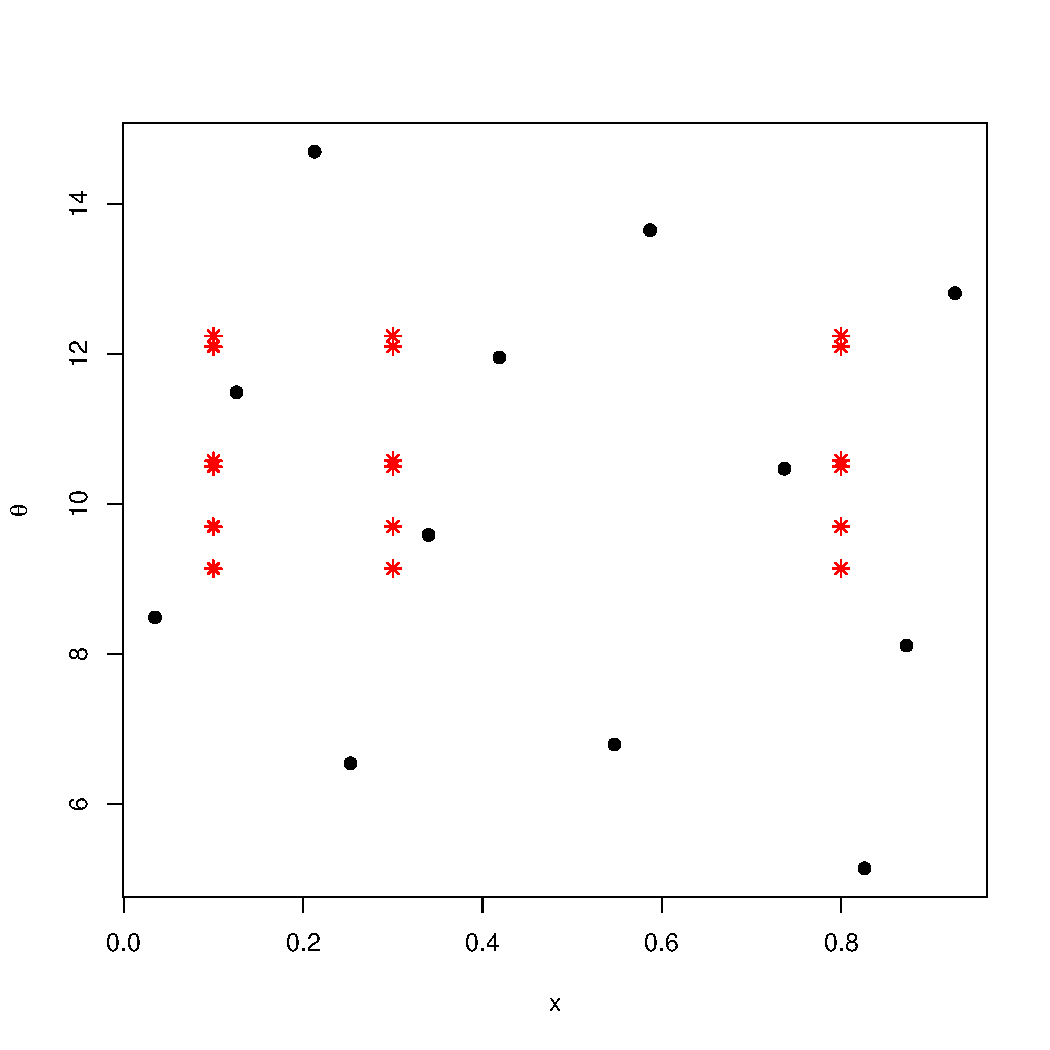
\includegraphics[scale=.3]{design_algo1.pdf}
  \end{figure}

 \end{center}
\end{frame}


\begin{frame}{Algorithm one at a time}
\textbf{\blue{Algorithm (step $\mathbf{k}\longrightarrow$ step $\mathbf{k+1}$) :}}
\bigskip
\begin{enumerate}
\item $\btheta_{k+1}=\argmax{\btheta}{EI_{k}(\btheta)}$,
\item $\Dc_{k+1}=\Dc_k \cup (\mathbf{x}^{\star},\btheta_{k+1})$ where $\mathbf{x}^{\star}\in\mathbf{X}^{F}=\big[\bxexp_1,\cdots,\bxexp_n\big]^{T}$,
\item $f(\Dc_{k+1})=f(\Dc_k)\cup \{f(\mathbf{x}^{\star},{\btheta_{k+1}})\}$,
\item $F^{D_{k+1}}=F|f(\Dc_{k+1})$,
\item $m_{k+1}:=\min{\{\mathbb{E}[SS_{k+1}(\btheta_1)],\cdots,\mathbb{E}[SS_{k+1}(\btheta_{k})],\mathbb{E}[SS_{k+1}(\btheta_{k+1})]\}}$.
\end{enumerate}

\medskip
\begin{center}
\fbox{\begin{tabular}{c}
\blue{\textbf{Only 1 simulation to compute $\mathbf{m_{k+1}}$!}}
\end{tabular}}
\end{center}

\medskip

where a criterion for step 2 is:
$\mathbf{x^{\star}}=\argmax{\bx\in\{\bxexp_1,\ldots,\bxexp_{\nexp} \}}\left(\,\,\,\frac{\text{Var}_F\big(F^{\Dc_k}(\bxexp_i,\btheta_{k+1})\big)}{\max\limits_{i=1,\cdots,n}\text{Var}_F\big(F^{\Dc_k}(\bxexp_i,\btheta_{k+1})\big)}
\times \frac{\text{Var}_{\btheta}(m^{k}(\bxexp_i,\btheta))}{\max\limits_{i=1,\cdots,n}\text{Var}_{\btheta}(m^{k}(\bxexp_i,\btheta))}\,\,\,\right)$ 

\end{frame}

 
\begin{frame}{Comparison full EI / EI one at a time}

%$\mathbf{X}^{f}=(0.1,0.2,0.3,0.4,0.5,0.6,0.7,0.8,0.9)$, $\Theta=[5,15]$

\begin{figure}[ht!]
\centering
\caption{\textit{\textbf{full EI}\,\,\,\,\,\,\,\,\,\,\,\,\,\,\,\,\,\,\,\,\,\,\,\,\,\,\,\,\,\,\,\,\,\,\,\,\,\,\,\,\,\,\,\,\,\,\,\,\,\,\,\,\,\,\,\,\,\,\,\,\,\,\,\,\,\,\,\,\,\,$\mathbf{EI}$ \textbf{OAT}}}
\vspace*{-0.7cm}
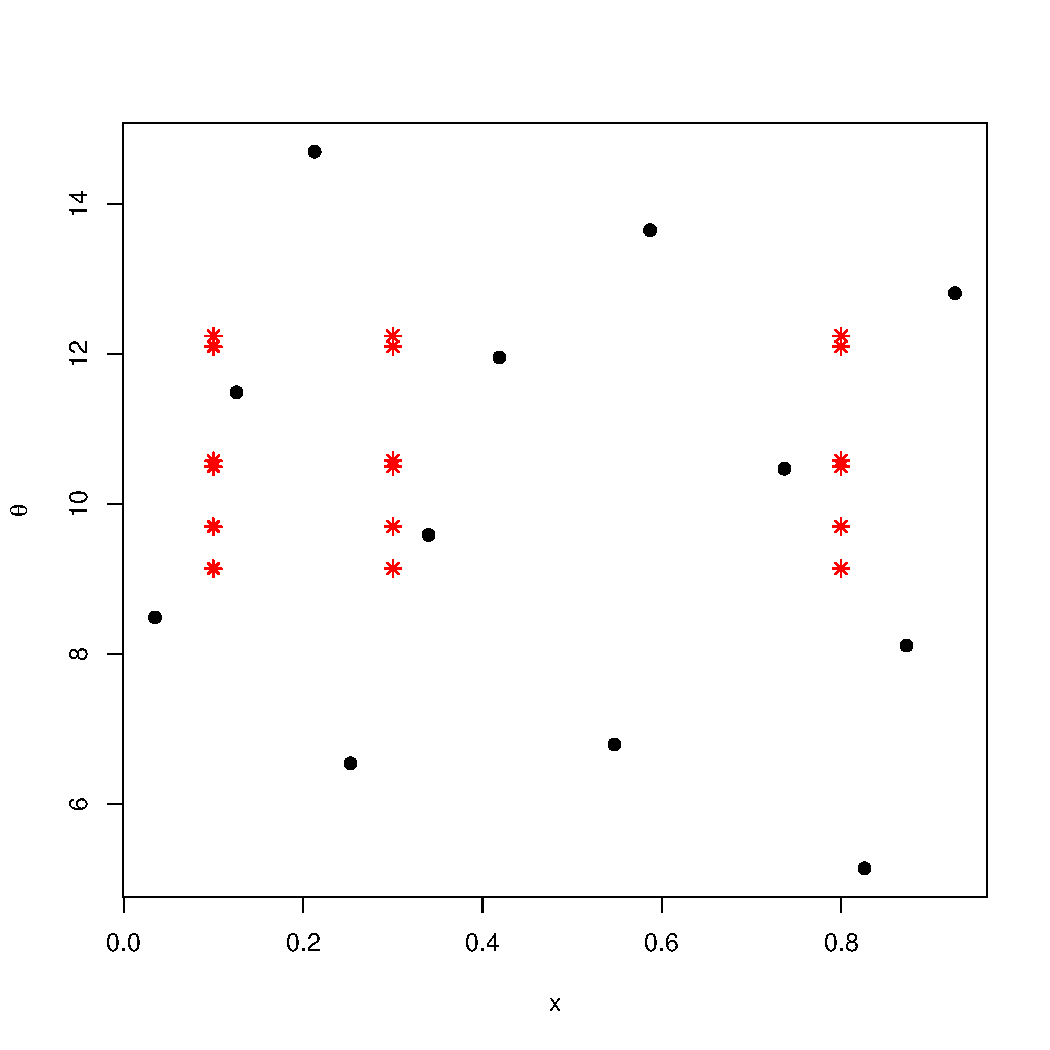
\includegraphics[scale=0.33]{design_algo1.pdf}
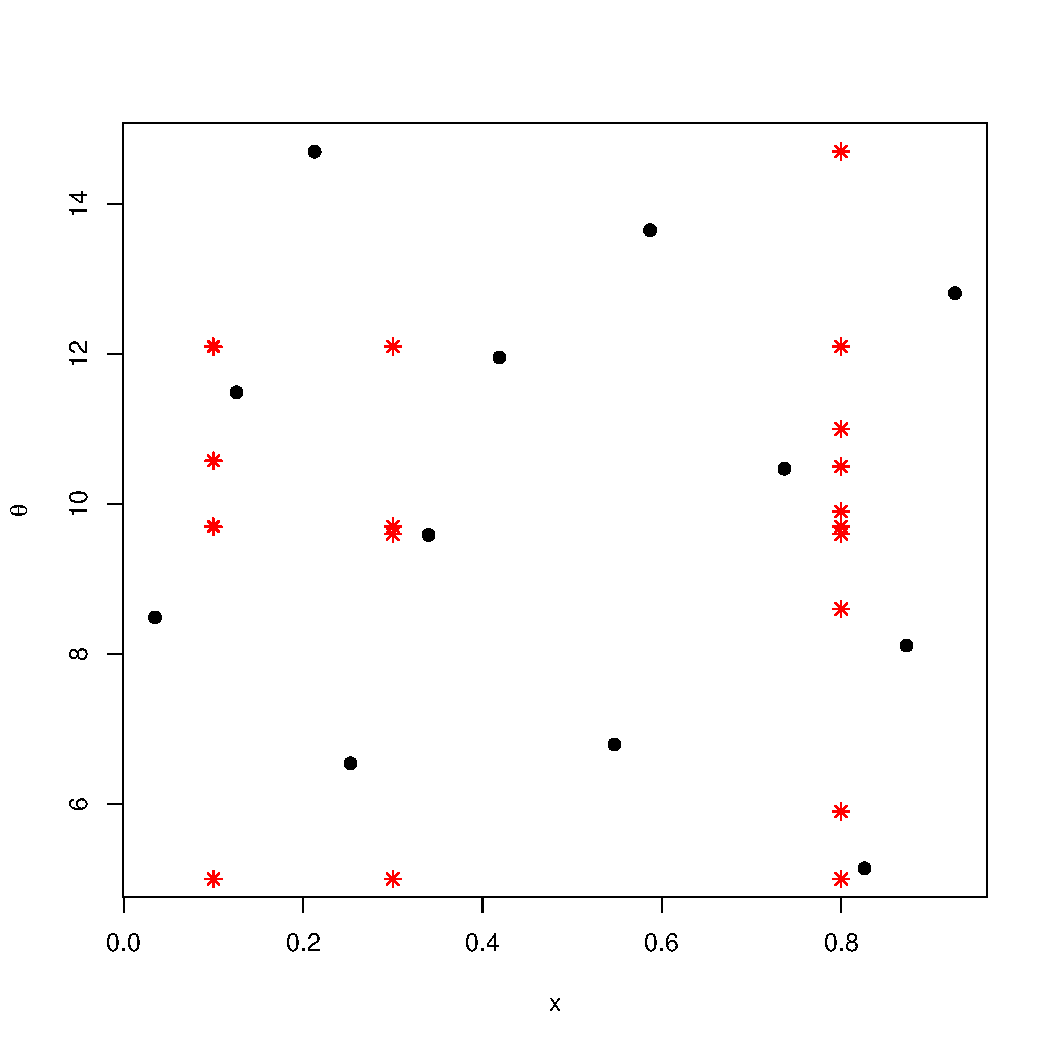
\includegraphics[scale=0.33]{design_algo2bis.pdf}
\end{figure}


\end{frame}



\begin{frame}
 \frametitle{}
 
 {\small
 \begin{beamerboxesrounded}{}
Recall that:
$$\pi(\btheta|\byexp)\propto \pi(\btheta)\cdot \exp(-SS(\btheta)/2\sigma^2)\,$$
is high where $\btheta\mapsto SS(\btheta)$ is small.  
 \end{beamerboxesrounded}
 \begin{multline}
 \nonumber
\label{KL_expression_dev}
%\textrm{KL}(\pi(\btheta|\mb{z}^f)||\pi^{C}(\btheta|\mb{z}^f,y(\Dc_M))=
\textrm{KL}\big(\pi(\btheta|\byexp)||\pi^{C}(\btheta|\byexp,f(\Dc_M))\big)=
\underbrace{K-K_M}_{(A)}+
\int_{\Theta}\pi(\btheta|\byexp)\underbrace{(C-C_M(\btheta))}_{(B)}\dd\btheta
\\+\frac{1}{2}\int_{\Theta}\pi(\btheta|\byexp)
\underbrace{\Big((\byexp-m(\bXexp,\btheta))^T\tilde\Sigma_{\byexp}^{-1}(\byexp-m(\bXexp,\btheta)))-SS(\btheta)/\sigma^2\Big)}_{(C)}\dd\btheta
\end{multline}
where $K$ and $K_M$ correspond to the normalizing constants:
\begin{equation}
\nonumber
K=-\log\left(\int_{\Theta}\mathcal{L}(\btheta;\byexp)\pi(\btheta)\right),\quad K_M=-\log\left(\int_{\Theta}
\mathcal{L}^C(\btheta;\byexp|f(\Dc_M))\pi(\btheta)\right),
\end{equation}
\begin{equation}
\nonumber
C=-\frac{n}{2}\log{\sigmaerr},\quad C_M(\btheta)=-\frac{1}{2}\log{|\tilde\Sigma_{\byexp}^{-1}|}=-\frac{1}{2}\log{(|\boldsymbol{\Sigma}_{exp,exp}(\bXexp,\btheta)+\sigmaerr\mb{I}_{\nexp})^{-1}|}.
\end{equation}
and
\begin{equation}
\nonumber
SS(\btheta)=\Vert \byexp - f(\bx,\btheta) \Vert^2.
\end{equation}
}
\end{frame}


\begin{frame}
 \frametitle{Sobol function}
 $\mb{x}\in\mathcal{X}=[0,1]^{3}$, $\btheta\in\Theta=[0,1]^{3}$
 \begin{equation*}
\label{sobol}
f_{\btheta}:\mb{x}\in\mathcal{X}\longrightarrow
f_{\btheta}(\mb{x})=\prod_{i=1}^{3}\frac{|4x_i-2|+\theta_i}{1+\theta_i}\,.
\end{equation*}
Field measurements $\mb{y}^f$ chosen according to a maximin LHD on $\mathcal{X}$ of size $n=60$. 
For $1\leq i\leq 60$, 
\begin{equation*}
y^f_i=f_{\btheta}(x^f_i)+\epsilon_i\,,
\end{equation*}
where ${\epsilon_i}\overset{i.i.d.}{\thicksim}
\mathcal{N}(0,0.05^{2})$ and $\btheta=(0.55,0.55,0.1)$.\\

\medskip
GPE is fitted with a constant mean $m_{\ms{\beta}}=m$ and a Matérn $5/2$ correlation function. 

\medskip
Prior distribution $\pi(\btheta)$ on $\Theta$:
\begin{equation*}
\pi({\btheta})\propto \mb{1}_{[0,1]^{3}}({\btheta}).
\end{equation*}
\end{frame}


\begin{frame}
 \frametitle{Designs}
 
 Number of simulations $M=150$.
 \\
 
 \bigskip
 
 Comparison of $4$ designs.
 
 
 \begin{enumerate}
  \item Maximin LHD in 6D: $\mathcal{X}\times\Theta=[0,1]^{6}$.
  
  \smallskip
  \item \textit{Restricted}-to-$\mb{X}^{f}$ maximin LHD.
  
  \smallskip
  \item Sequential designs OAT with GPE variance criterion for choosing $\mathbf{x}_{k+1}^{\star}$.
  
  
  \smallskip
  \item Sequential designs OAT with trade-off (GPE-variance, variability of $f$ w.r.t. $\mb{x}$) (variance criterion for choosing $\mathbf{x}_{k+1}^{\star}$.
  
 
 \end{enumerate}

 
 Sequential designs based on an initial design with $M_0=75$ points chosen as a \textit{Restricted}-to-$\mb{X}^{f}$ maximin LHD.
\end{frame}


\begin{frame}
 \frametitle{Marginal posterior distributions}
 
 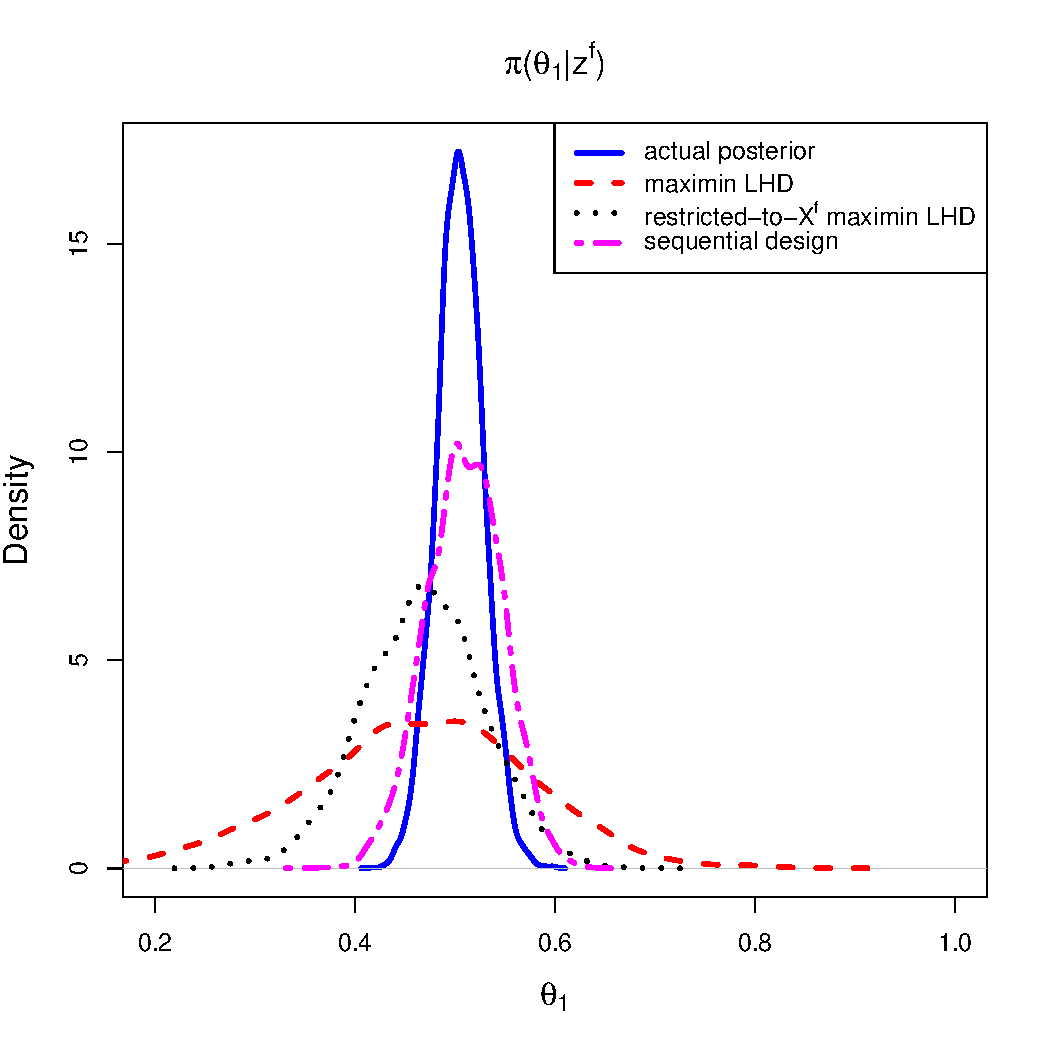
\includegraphics[scale=0.22]{ExSobold6_marg1_150.pdf}
  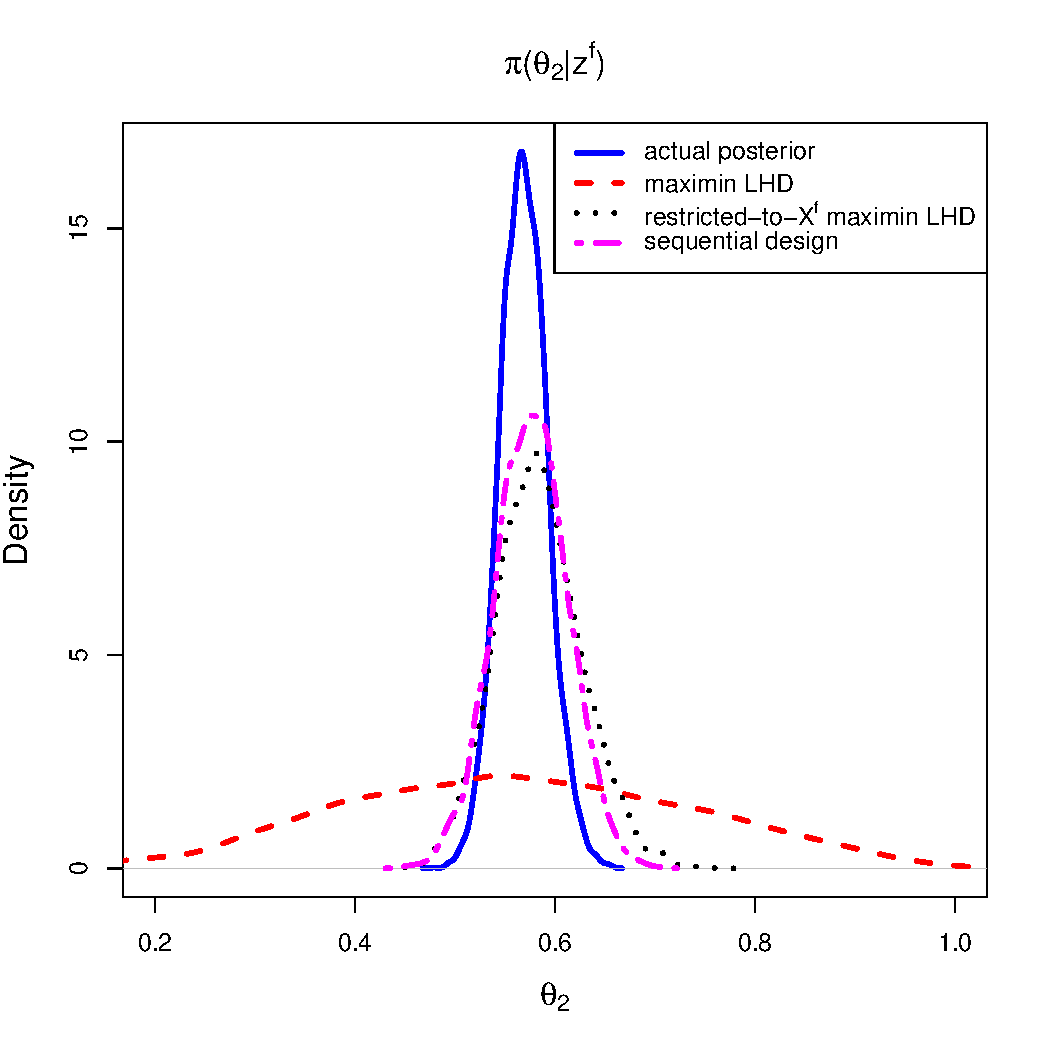
\includegraphics[scale=0.22]{ExSobold6_marg2_150.pdf}\\
 
 \vspace{-.2cm}
 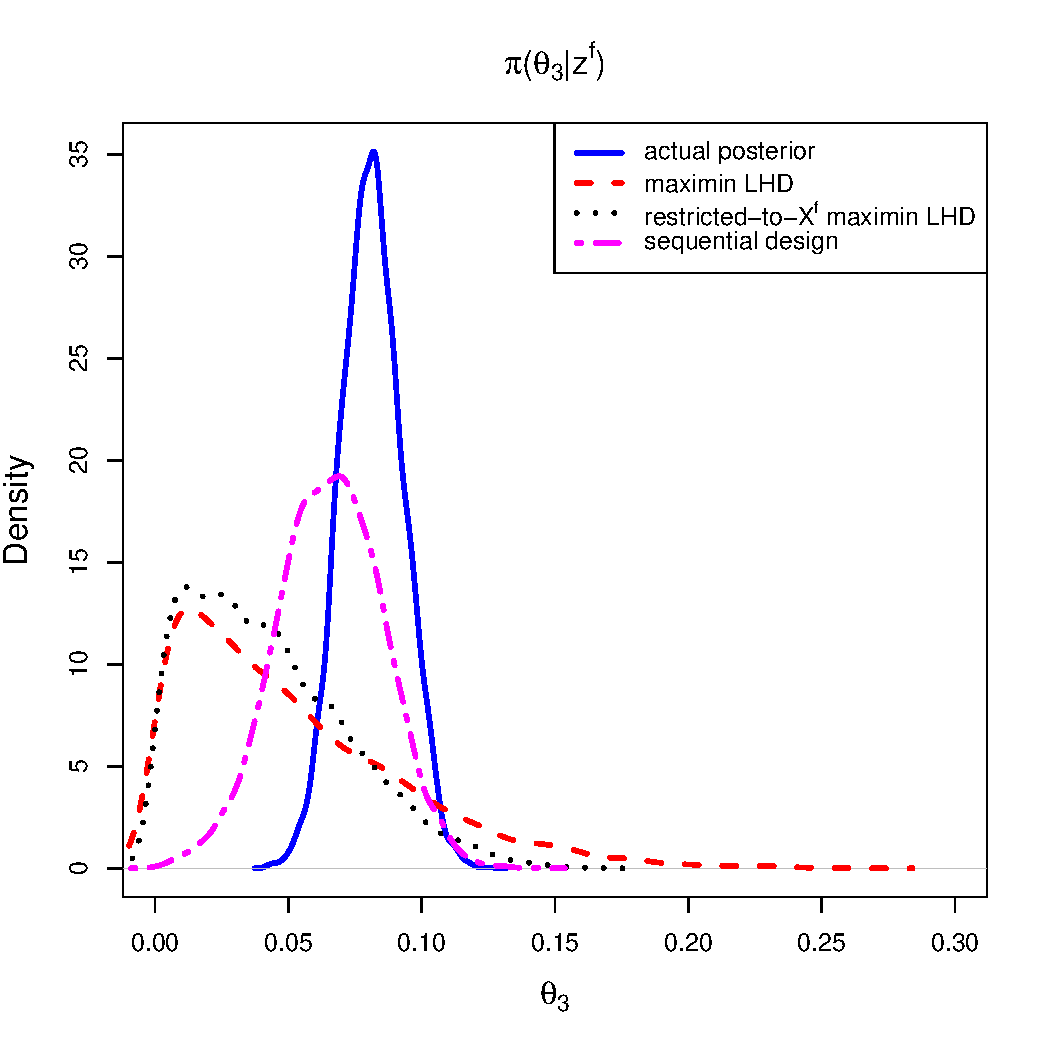
\includegraphics[scale=0.22]{ExSobold6_marg3_150.pdf}
 
 
\end{frame}


\begin{frame}
 \frametitle{see also}
 
 \cite{surer2023sequential}
\end{frame}


\bibliographystyle{apalike}
\bibliography{biblio}


\end{document}

